\section{Appendix}

In the following, we describe our previous work that was done towards considering safe reinforcement learning. 
Precisely, we were motivated by the lack of safety guarantees and the use of symbolic reasoning towards incorporating 
safety properties from a verified safe controller (SC) i.e. a declarative language module to compute safe and unsafe states. 
Those safety states are computed during training, thus ensuring that no unsafe states are explored 
by the RL. The general idea was to allow training in the real-world, thus taking away the need for simulation. Our proposed RL+SC architecture is shown in Figure \ref{fig:rlsc}.


\begin{figure}[H]
  \centering
  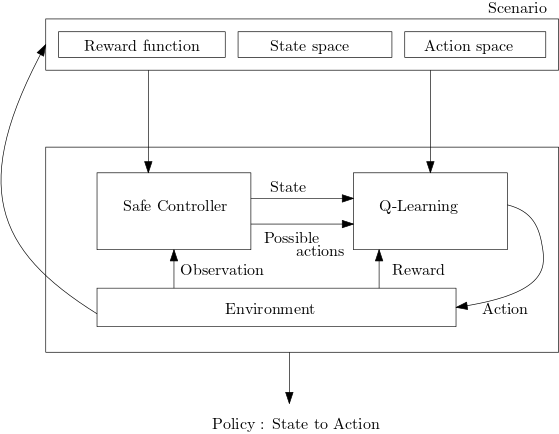
\includegraphics[scale=0.5]{rlsc.png}
  \caption{Overview of the proposed solution}
  \label{fig:rlsc}
\end{figure}

\begin{enumerate}
  \item The environment sends the observation to the SC. 
  \item The SC computes the state from the observation, thus keeping only 
        ground facts that uphold the \emph{Markov Property} (see Definition 9.1). 
  \item The SC also computes the set of possible actions $A$ that ensure that no unsafe states is 
        reached. This is done by searching for possible configurations that follow a (state, action) pair over 
        all possible actions from the action spaces. 
  \item The state and set of possible actions is sent to the RL algorithm, thus only allowing 
        the agent to choose from the set actions. 
  \item Next steps follow from the RL basic routine from Figure \ref{fig:rl}
\end{enumerate}

The implementation can be found in the thesis corresponding github under the rl-implementation folder\footnote{https://github.com/natvern/Thesis}.
For our case study, we chose the vehicle platooning problem. The setting is as follows; two vehicles, one leader and one follower. Their goal is to 
minimize the gap between them while ensuring that they do not crash. 

\medskip

We then present our preliminary results before arguing for the issues with our approach. 

\begin{figure}[H]
  \centering
  \begin{minipage}{.5\textwidth}
    \centering
    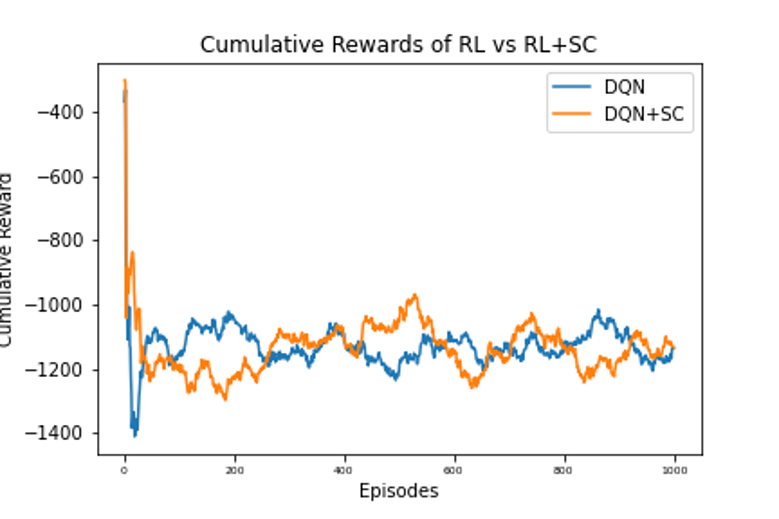
\includegraphics[width=1\linewidth]{appendixopt.png}
    \captionof{figure}{Cumulative Rewards of RL vs. RL+SC}
    \label{fig:optsc}
  \end{minipage}%
  \begin{minipage}{.5\textwidth}
    \centering
    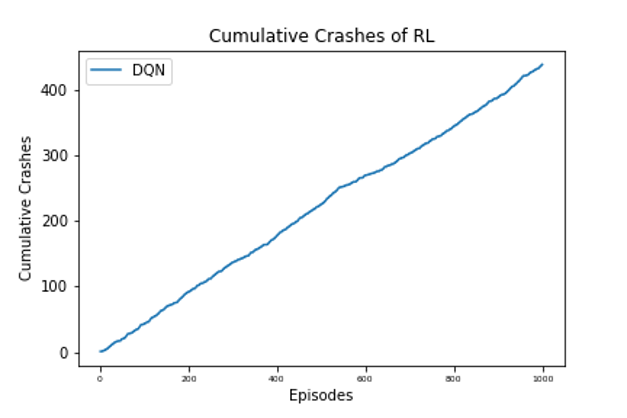
\includegraphics[width=1\linewidth]{appendixcrash.png}
    \captionof{figure}{Cumulative Crashes of RL during Training}
    \label{fig:crashsc}
  \end{minipage}
\end{figure}
  
The graph in Figure \ref{fig:optsc} shows the cumulative rewards of the basic RL implementation without
the safe controller (blue line) vs. the RL+SC implementation (orange line). As evident in the cumulative rewards, all are negative. This is because of our reward function choice 
that only punishes for distances not equal to the desired gap. Thus, learning is not optimal. We can however see that the cumulative rewards of both implementation does not change by a significant 
amount. The graph in Figure \ref{fig:crashsc} shows 
the number of crashes of the basic RL during training. We can easily deduce from the linear graph that the RL without the SC never learns not to crash.


\begin{definition}[Markov Property]
  The next state only depends on the value of the current state. In other words, only the present can affect the future. 
  In terms of our state vector, this means that given $S_t$, I only need the features in $S_t$ to predict $S_{t+1}$.
\end{definition}

\subsection{Issues with the safe RL approach}
\begin{itemize}
  \item The simplicity of our problem setting does not showcase the need for a SC as we only consider two vehicles on an x-axis. 
  \item Though ensuring safety guarantees during training theoretically takes away the need for a simulation, in practice, the uncertainties 
        of the real world cannot be all predicted. This results in a handful of safety properties that might be guaranteed, not enough to allow sensitive cyber-physical systems 
        to be trained using RL in the real world. 
  \item If an oracle existed that was able to predict all uncertainties of the real world, this oracle could then be used to solve the optimization problem 
        deterministically without the need for RL. 
  \item Depending on the SC implementation, safety guarantees can be too strict thus completely destroying optimality. Consider a SC that only allows a car not to move. 
        Though it guarantees that no crashes happen, it is also too strict, thus going against the goal of the agent. 
  
\end{itemize}


